\documentclass{article}
\usepackage{graphicx}
\usepackage[utf8]{inputenc}
\usepackage[T1]{fontenc}
\usepackage{fouriernc}
\usepackage[margin=1in]{geometry}
\usepackage{amsmath}
\begin{document}

\begin{titlepage}
	\centering 
	\scshape
	\vspace*{\baselineskip}
	\rule{\textwidth}{1.6pt}\vspace*{-\baselineskip}\vspace*{2pt}
	\rule{\textwidth}{0.4pt} 
	\vspace{0.75\baselineskip}
	
	{\Large CS 374 : Computational and Numerical Methods \\\vspace{0.75\baselineskip} Set 6}
	\vspace{0.75\baselineskip}
	
	\rule{\textwidth}{0.4pt}\vspace*{-\baselineskip}\vspace{3.2pt} 
	\rule{\textwidth}{1.6pt}
	
	\vspace{2\baselineskip}  
	The Bisection Method
	
	\vspace*{3\baselineskip}
	
	\vspace{0.5\baselineskip} %originally 0.5
	
	{\scshape\large Purvil Mehta (201701073) \\ Bhargey Mehta (201701074) \\} 
	
	\vspace{1\baselineskip} 
	
	\textit{Dhirubhai Ambani Institute of Information and Communication Technology \\ Gandhinagar\\} 
	\vspace*{2\baselineskip}
	\today


\end{titlepage}

\newpage
\tableofcontents
\newpage
\section{Linear Interpolation of $f(x) = \sqrt{x}$}
Carry out the Lagrange linear interpolation between (1,1) and (4,2). Plot the linear interpolation function together with $f(x) = \sqrt{x}$.
\subsection{Plots}
\begin{figure}[!h]
    \centering
    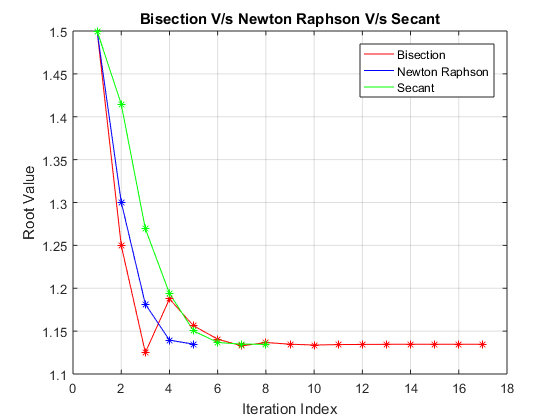
\includegraphics[scale=0.55]{1_1.png}
    \caption{Linear Interpolation of $f(x) = \sqrt{x}$}
\end{figure}
\subsection{Equations}
The general formula for the first order Lagrange's Interpolation is defined as,
$$p_1(x) = \frac{x-x_1}{x_0-x_1}y_0 + \frac{x-x_0}{x_1-x_0}y_1$$
\subsection{Observation}
By looking at the graph above we say that , the more order in the Lagrange's Equation we use,the less and less error we get in the approximation. 


\newpage
\section{Linear Interpolation of $f(x) = e^{x}$}
Carry out a Lagrange linear interpolation for (0.82, 2.270500) and (0.83, 2.293319). Extend your study with a Lagrange quadratic polynomial using (0.84, 2.316367). Compare your polynomials with the function $y = e^x$, plotting all of them on the same graph.
\subsection{Plots}
\begin{figure}[!h]
    \centering
    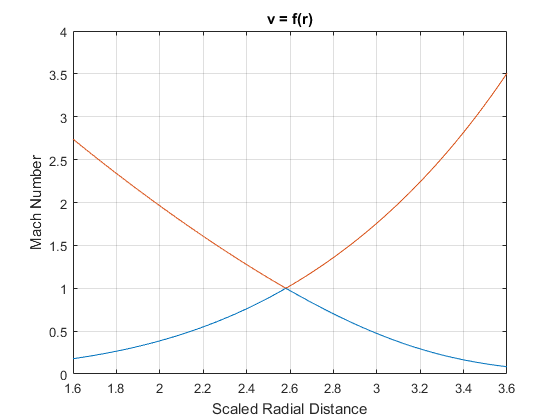
\includegraphics[scale=0.36]{2_1.png}
    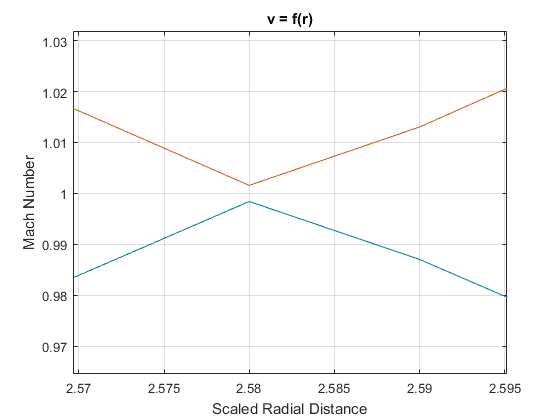
\includegraphics[scale=0.36]{2_2.png}
    \caption{Linear Interpolation of $f(x) = e^{x}$}
\end{figure}
\subsection{Equations}
The general formula for the first order and second order  Lagrange's Interpolation is defined as,
$$p_1(x) = \frac{x-x_1}{x_0-x_1}y_0 + \frac{x-x_0}{x_1-x_0}y_1$$
$$p_2(x) = \frac{(x-x_1)(x-x_2)}{(x_0-x_1)(x_0-x_2)}y_0 + \frac{(x-x_0)(x-x_2)}{(x_1-x_0)(x_1-x_2)}y_1 + \frac{(x-x_1)(x-x_0)}{(x_2-x_1)(x_2-x_0)}y_2$$
By putting the values of $x_0 = 0.82$ ,$x_1 = 0.83$,$x_2 = 0.84$,$y_0 = 2.270500$,$y_1 = 2.293319$ and $y_2 = 2.316367$ in the above equation we get approximation as ,
$$p_1(x) = -(x-0.83)(0.22705) + (x-0.83)(0.2293319)$$
$$p_2(x) = (x-0.83)(x-0.84)(0.022705) - (x-0.82)(x-0.84)(0.02293319) - (x-0.83)(x-0.82)(0.02316367)$$
\subsection{Observation}
\begin{itemize}
   \item By looking at the graph above we say that , the more order in the Lagrange's Equation we use,the less and less error we get in the approximation.
   \item The quadratic and linear interpolation around the given data points are almost the same.
\end{itemize}

\newpage
\section{Interpolation using Lagrange's Method and Newton's Method}
Construct a quadratic Lagrange polynomial using the points (0,-1), (1,-1) and (2, 7). Plot your result. Extend this entire exercise with Newton’s divided-difference quadratic
polynomial and compare the two methods.
\subsection{Plots}
\begin{figure}[!h]
    \centering
    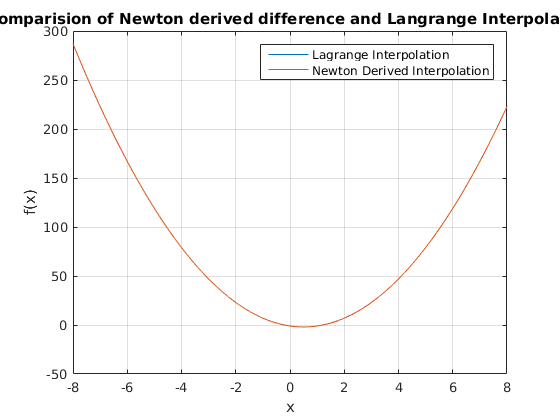
\includegraphics[scale=0.6]{3_1.png}
    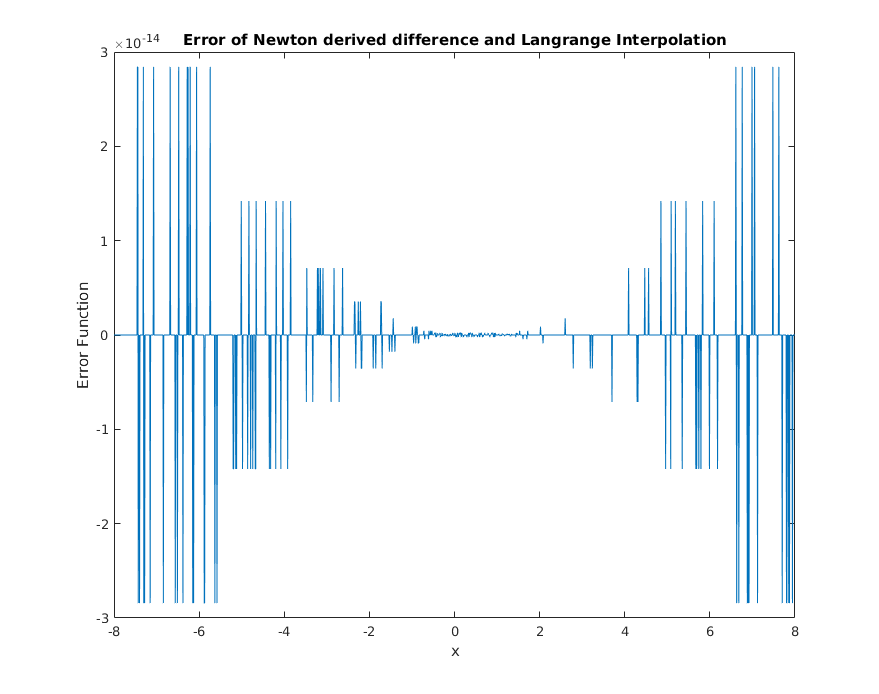
\includegraphics[scale=0.4]{3_2.png}
    \caption{Quadratic Interpolation of Newton's Derived Difference and Lagrange's Method}
\end{figure}
\subsection{Equations}
The general formula for the first order and second order  Lagrange's Interpolation is defined as,

$$p_2(x) = \frac{(x-x_1)(x-x_2)}{(x_0-x_1)(x_0-x_2)}y_0 + \frac{(x-x_0)(x-x_2)}{(x_1-x_0)(x_1-x_2)}y_1 + \frac{(x-x_1)(x-x_0)}{(x_2-x_1)(x_2-x_0)}y_2$$
$$n_1(x) = y_0 + (x-x_0)f[x_0,x_1]$$
$$n_2(x) = n_1(x) + (x-x_0)(x-x_1)f[x_0,x_1,x_2]$$
where,
$$f[x_0,x_1] = \frac{f(x_1)-f(x_0)}{x_1-x_0}$$
$$f[x_0,x_1,x_2] = \frac{f[x_1,x_2]-f[x_0,x_1]}{x_2-x_0}$$

\subsection{Observation}
\begin{itemize}
   \item The error between two method is very less around $10^{-14}$.
   \item By looking at the graph above we say that , the Lagrange's Interpolation and Newton's Derived Difference Interpolation tends to the unique function and hence we got similar looking graph in both cases.
\end{itemize}



\section{Interpolation using Lagrange's Method and Newton's Method}
For given data points,
\begin{itemize}
    \item $f(3.35) = 0.298507$
    \item $f(3.40) = 0.294118$
    \item $f(3.50) = 0.285714$
    \item $f(3.60) = 0.277778$
\end{itemize}
(a) Produce Lagrange polynomials of the linear, quadratic and cubic orders with increasing values of x.
(b) Produce Newton’s divided-difference polynomials of all the three foregoing orders.
(c) Plot the results of both methods on the same graph and compare them with the function $y = \frac{1}{x}$. Also comment on the respective computational advantages of the two methods above.
\subsection{Plots}
\begin{figure}[!h]
    \centering
    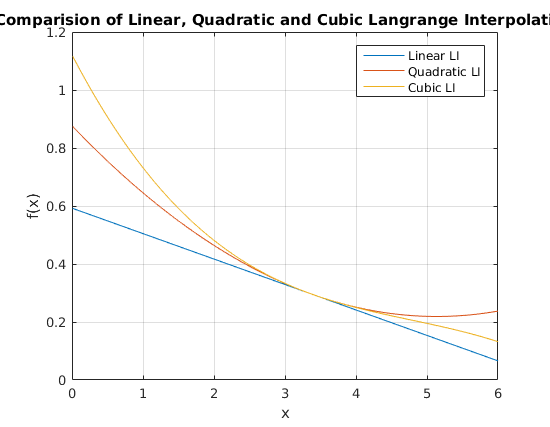
\includegraphics[scale=0.5]{4_a_1.png}
    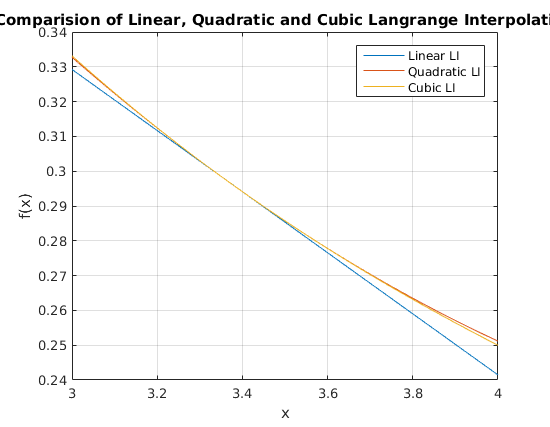
\includegraphics[scale=0.5]{4_a_2.png}
    \caption{Interpolation using Lagrange's Method}
\end{figure}
\newpage
\begin{figure}[!h]
    \centering
    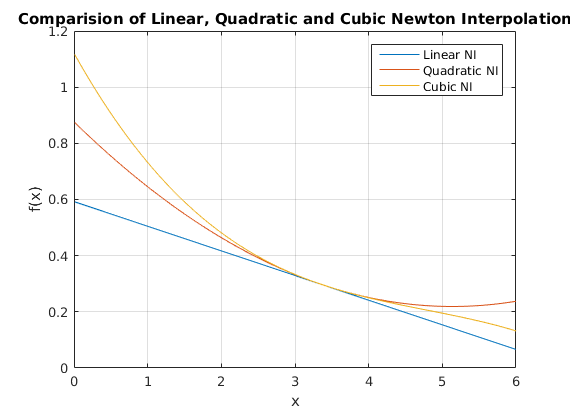
\includegraphics[scale=0.5]{4_b_1.png}
    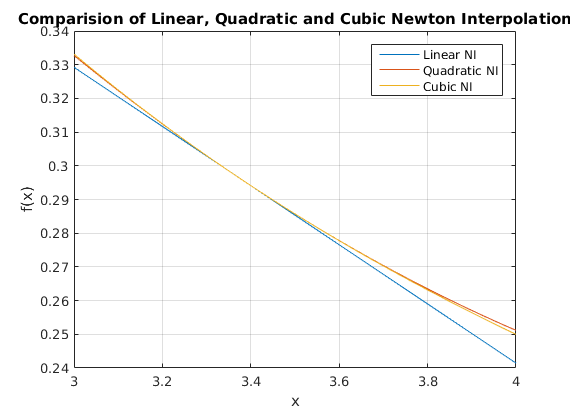
\includegraphics[scale=0.5]{4_b_2.png}
    \caption{Interpolation using Newton's Derived Difference}
\end{figure}
\begin{figure}[!h]
    \centering
    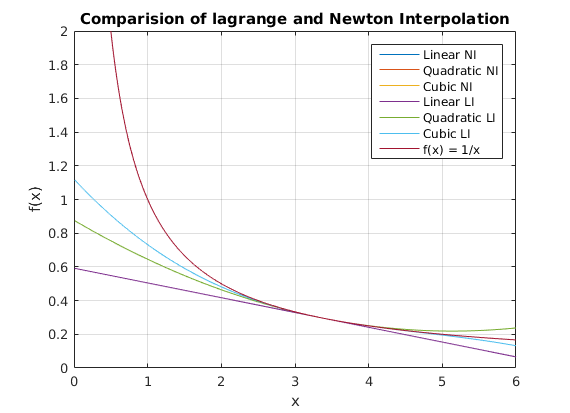
\includegraphics[scale=0.5]{4_c_1.png}
    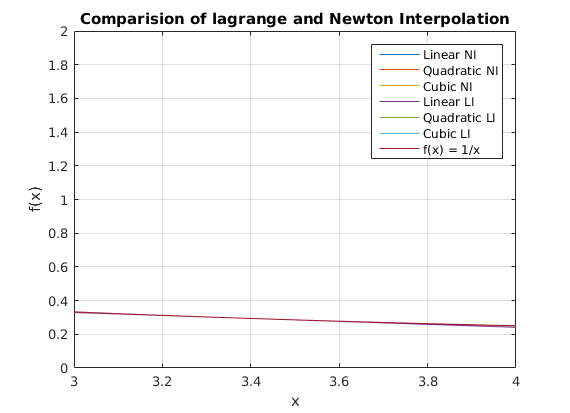
\includegraphics[scale=0.5]{4_c_2.png}
    \caption{Comparison with Actual Function $f(x) = \exp{x}$}
\end{figure}
\subsection{Equations}
The general formula for the first order and second order  Lagrange's Interpolation is defined as,

$$p_3(x) = \frac{(x-3.40)(x-3.50)(x-3.60)}{(-0.05)(-0.15)(-0.25)}(0.298507) + \frac{(x-3.35)(x-3.50)(x-3.60)}{(-0.05)(-0.10)(-0.20)}(0.294118) +$$$$ \frac{(x-3.35)(x-3.40)(x-3.60)}{(-0.05)(-0.10)(-0.10)}(0.295778) +
\frac{(x-3.35)(x-3.50)(x-3.40)}{(-0.25)(-0.20)(-0.10)}(0.298507)$$
$$n_1(x) = y_0 + (x-x_0)f[x_0,x_1]$$
$$n_2(x) = n_1(x) + (x-x_0)(x-x_1)f[x_0,x_1,x_2]$$
$$n_3(x) = n_2(x) + (x-x_0)(x-x_1)(x-x_2)f[x_0,x_1,x_2,x_3]$$
where,
$$f[x_0,x_1] = \frac{f(x_1)-f(x_0)}{x_1-x_0}$$
$$f[x_0,x_1,x_2] = \frac{f[x_1,x_2]-f[x_0,x_1]}{x_2-x_0}$$
$$f[x_0,x_1,x_2,x_3] = \frac{f[x_1,x_2,x_3] - f[x_0,x_1,x_2]}{x_3-x_0}$$
\subsection{Observation}
\begin{itemize}
   \item By looking at the graph above we say that , the Lagrange's Interpolation and Newton's Derived Difference Interpolation tends to the unique function in each and every order and hence we got similar looking graph in both cases.
   \item Computationally , the Lagrange's method would be less expensive as compared as the Newton's method due to it's recursive nature.
\end{itemize}

\section{Interpolation using Lagrange's Method and Newton's Method}
For given data points,
\begin{itemize}
    \item $f(0) = 2.5$
    \item $f(1) = 0.5$
    \item $f(2) = 0.5$
    \item $f(2.5) = 1.5$
    \item $f(3) = 1.5$
    \item $f(3.5) = 1.125$
    \item $f(4) = 0$
\end{itemize}
(a) Interpolate successive points by straight line segments. This is known as piece wise linear interpolation.
(b) On each of the three following sub intervals of x [0, 2], [2, 3] and [3, 4] interpolate using both Lagrange’s quadratic polynomial and Newton’s divided-difference interpolation polynomial.
(c) Plot the results of both methods covering all the three sub intervals on the same graph and compare them.
\subsection{Plots}
\begin{figure}[!h]
    \centering
    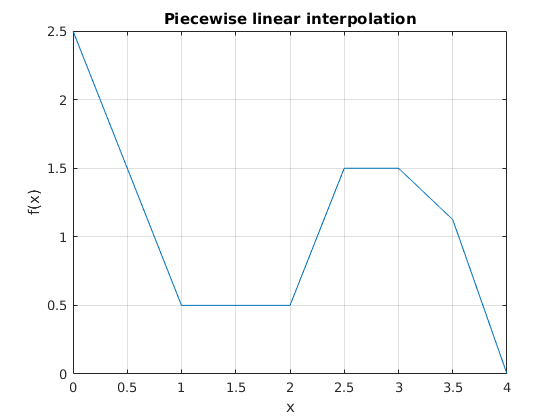
\includegraphics[scale=0.8]{5_a_1.png}
    \caption{Piece wise Linear Interpolation}
\end{figure}
\newpage
\begin{figure}[!h]
    \centering
    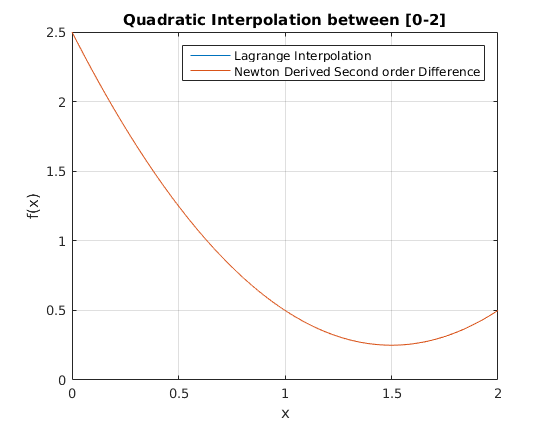
\includegraphics[scale=0.56]{5_b_1.png}
    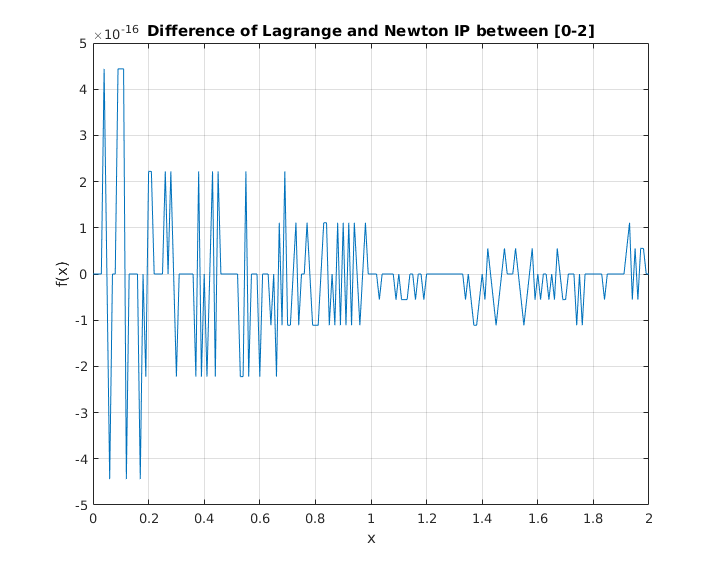
\includegraphics[scale=0.43]{5_b_2.png}
    \caption{Interpolation between [0-2]}
\end{figure}
\begin{figure}[!h]
    \centering
    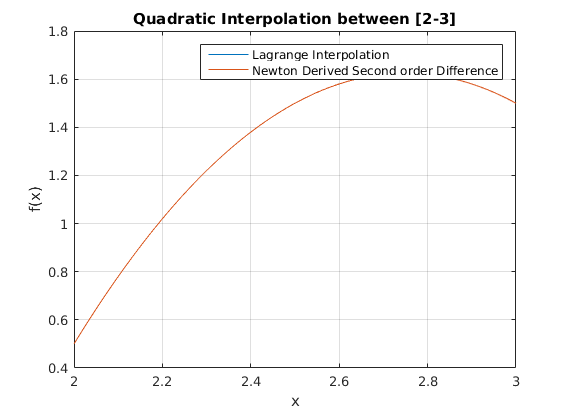
\includegraphics[scale=0.55]{5_b_3.png}
    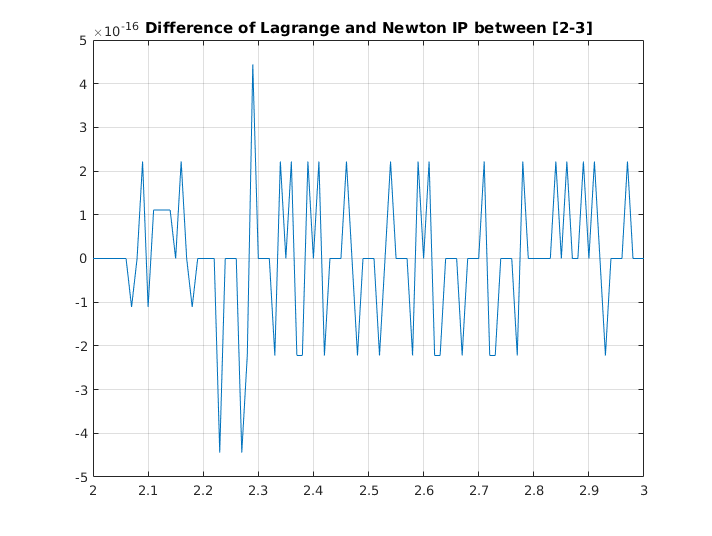
\includegraphics[scale=0.43]{5_b_4.png}
    \caption{Interpolation between [2-3]}
\end{figure}
\begin{figure}[]
    \centering
    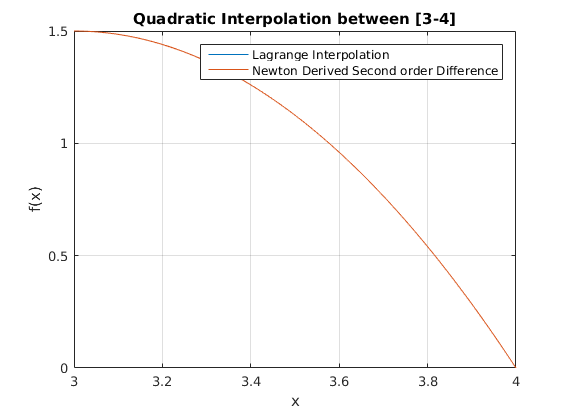
\includegraphics[scale=0.55]{5_b_5.png}
    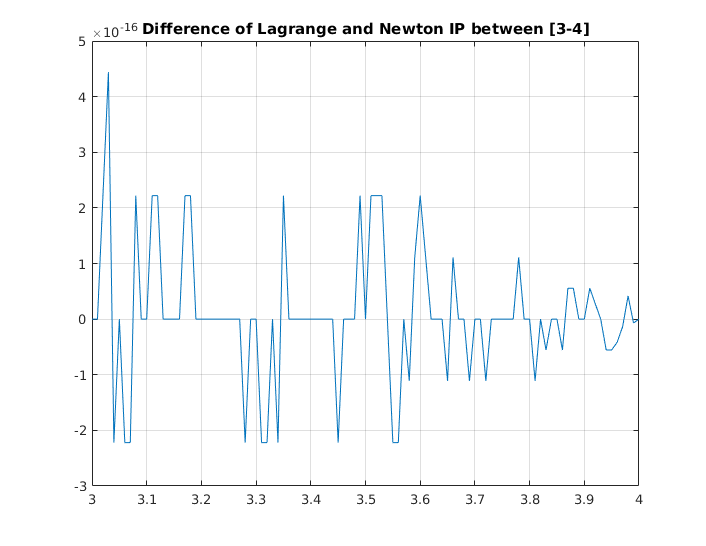
\includegraphics[scale=0.43]{5_b_6.png}
    \caption{Interpolation between [3-4]}
\end{figure}
\begin{figure}[!h]
    \centering
    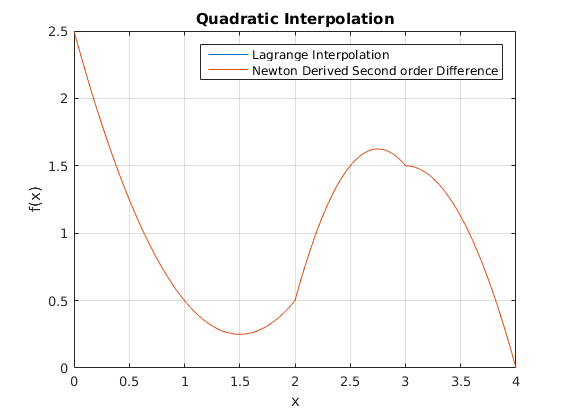
\includegraphics[scale=0.5]{5_b_7.png}
    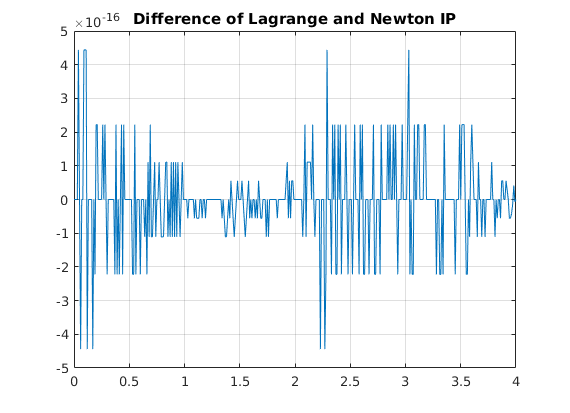
\includegraphics[scale=0.5]{5_b_8.png}
    \caption{Interpolation between [0-3]}
\end{figure}
\subsection{Observation}
\begin{itemize}
   \item By looking at the graph above we say that , the Lagrange's Interpolation and Newton's Derived Difference Interpolation tends to the unique function in each and every order and hence we got similar looking graph in both cases.
\end{itemize}

\end{document}